\documentclass{report}
\usepackage[margin=1in]{geometry}
\usepackage{setspace}
\usepackage{times}
\title{
	\textsc{ \small
		Washington State University \\
		School of Electrical Engineering and Computer Science \\
		EE 352, Electrical Engineering Laboratory
	} \\
	{\textsc{\small Lab \#8}} \\
	MOSFET Amplifier Circuits
}

\author{
	Name: Kevin Evans
}
\date{Due Date: March 31, 2020}


% start sections at 1 with subsections to 1.1, 1.2...
\renewcommand{\thesection}{\arabic{section}}

%alias for vpp/rms
\newcommand{\pp}{_{pp}}
\newcommand{\rms}{_{rms}}
\newcommand{\Vpp}{\V\pp}
\newcommand{\Vrms}{\V\rms}

\usepackage{siunitx}
\usepackage{threeparttable}
\usepackage{booktabs}
\usepackage{multirow}
\usepackage{graphicx}
\usepackage{float}
\usepackage{amssymb,amsmath}
\usepackage{physics,cancel}
\usepackage{listings}
\usepackage{caption,subcaption} %multiline captions; subfigures
\begin{document}
\maketitle

\section*{Lab Overview}
% what was the lab about and the outcome?
The purpose of this lab was to explore the various properties of MOSFET transistors and their use in amplifier circuits. We will design and validate the common source amplifier circuit design using the ZVN2110A NFET transistor. Next, we will build the current mirror circuit using matched transistors on the CD4007 IC. Then, we will build an inverter with the same CMOS chip.
%%%%%%%%%%%%%%%%%%%%%%%%%%%%%%%%%%%%%%%%%%%%%%%%%%%%%%%%%%%%%
\section{Single stage common source amplifier}

\subsection{Purpose}
% purpose of the experiment and its specs and/or design requirements
The purpose of this experiment is to design a common source amplifier under the listed requirements. We will use the ZVN2110A NMOS transistor to amplify an AC input signal. The design requirements are listed below in Table \ref{table:exp1specs}.
 
\subsection{Theoretical background}
% background and its theory of operation, circuit diagrams, the main equations, results from the prelab
In this experiment, we will design a common source amplifier using the ZVN2110A transistor. We are to follow the common source amplifier circuit shown in Figure \ref{fig:exp1ckt} and to determine the component values to reach the required amplifier specifications, shown in Table \ref{table:exp1specs} below.
\begin{table}[h]
	\caption{Required specifications of the amplifier}
	\label{table:exp1specs}
	\centering
	\begin{tabular}{lll}
		\toprule
		Specification & Symbol & Value \\
		\midrule
		Load resistance & $R_L$ & $\SI{100}{\kohm}$ \\
		Input resistance & $R_i$ & $> \SI{200}{\kohm}$ \\
		Mid-band gain & $G_V$ & $-\SI{50}{\V/\V} \pm 20 \%$ \\
		Supply voltage & $V_{DD}$ & $\SI{15}{\V}$ \\
		Circuit capacitors & $C_G$ & \SI{10}{\micro\farad} \\
		& $C_S$ & \SI{47}{\micro\farad} \\
		& $C_D$ & \SI{10}{\micro\farad} \\
		\bottomrule
	\end{tabular}
\end{table}

In order to achieve these specifications, the resistor values must be chosen appropriately. To accomplish this, we begin by finding the small signal approximation, shown in Figure \ref{fig:exp1cktac}. In this circuit, both the input resistors $R_1$ and $R_2$ are brought to AC ground, as $V_{DD}$ is DC-only. The AC input and output resistances then become \begin{align}
	R_\mathrm{in} & = R_1 \parallel R_2 \\
	R_\mathrm{o} & = R_D \parallel R_L \parallel r_o \label{eq:exp1Ro}
\end{align}
The amplifier gain is then specified by the dependent source and the transconductance is parameterized by the specifications of the transistor, \begin{align}
	G_V & = -g_m R_\mathrm{o} \label{eq:exp1gain} \\
	g_m & = \sqrt{2 k_n I_D } = k_n \left(V_{GS} - V_T\right) \label{eq:exp1gm}
\end{align}
At DC, the equivalent circuit is shown in Figure \ref{fig:exp1cktdc}. This is achieved as the capacitors act as an open circuit for a DC input. From the DC circuit, we can determine the DC bias voltage at the gate using a simple voltage divider, \begin{align}
	V_G & = \frac{R_2}{R_1 + R_2} V_{DD} \label{eq:exp1vg}
\end{align}
From the previous lab, we found approximate values for $V_T$, $K_n$, and $\lambda$. If we take a drain current $I_D \approx \SI{0.3}{\mA}$, we can find the transconductance $g_m$ and equivalent dynamic resistance $r_o$,
\begin{align*}
	g_m & = \sqrt{2 k_n I_D} \approx \SI{3.464}{\mA/\V} \\
	r_o & = \frac{1}{\lambda I_D} \approx \SI{333.3}{\kohm}
\end{align*}
Then, from \eqref{eq:exp1gain}, the total output resistance can be found, and using \eqref{eq:exp1Ro}, we can find $R_D$ \begin{align*}
	R_o & = \frac{G_V}{-g_m} = \frac{50}{\SI{3.464}{\mA/\V}} = \SI{14.433}{\kohm} \\
	R_D & =  \left(R_o^{-1} - r_o^{-1} - R_L^{-1}\right)^{-1} = \SI{17.8}{\kohm} \approx \SI{20}{\kohm}
\end{align*}
For this value of $R_D$, we can determine the voltage drop across the resistor at the current \SI{0.3}{\mA} and find the drain voltage,
\[ V_D = V_{DD} - I_D R_D = \SI{9}{\V}\]
Now we can determine the gate voltage using \eqref{eq:exp1gm} and the transconductance found earlier. \begin{align}
	g_m & = k_n \left(V_{GS} - V_T\right) \notag \\
	V_{GS} & = \frac{g_m}{k_n} + V_T \notag \\
	V_G & = \frac{g_m}{k_n} + V_T + V_S
\end{align}
If we choose the source voltage $V_S$ of \SI{3}{\V}, we find the source resistance and gate voltage to as \begin{align*}
	R_S & = \SI{10}{\kohm} \\
	V_G & = \SI{4.873}{\V}
\end{align*}
Then, if we choose $R_1$ to be \SI{1}{\Mohm}, we can use \eqref{eq:exp1vg} to find $R_2 \approx \SI{470}{\kohm}$.
\begin{figure}[h]
	\centering
	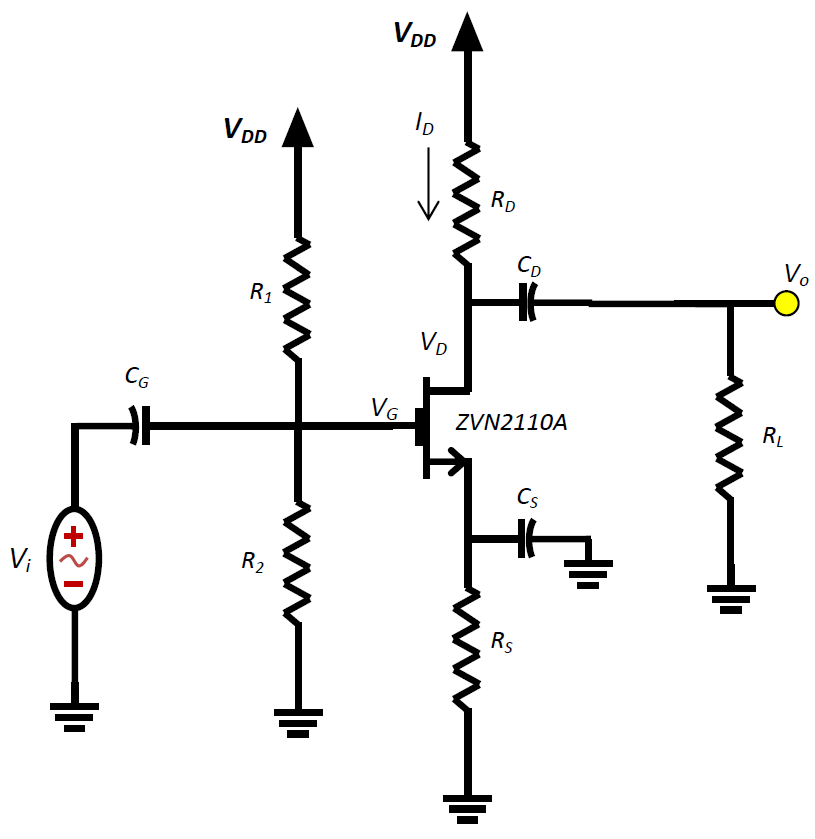
\includegraphics[width=0.5\linewidth]{exp1ckt}
	\caption{The common source amplifier circuit used in Experiment 1.}
	\label{fig:exp1ckt}
\end{figure}

The amplifier circuit was simulated using PSPICE within OrCAD using the component values found previously. The circuit drawn is shown in Figure \ref{fig:exp1pspiceckt} with the NMOS transistor modeled using $V_T \approx 1.7$, $K_n \approx 0.02$, and $V_A \approx 100$. An AC sweep simulation was done from \SI{100}{\Hz} to \SI{10}{\MHz} with the plot of the results shown in Figure \ref{fig:exp1spice}. This resulted in a mid-band gain of approximately \SI{57}{\V/\V}, within the 20\% margin in the specifications.

\begin{figure}[H]
	\centering
	\begin{subfigure}{0.55\textwidth}
		\centering
		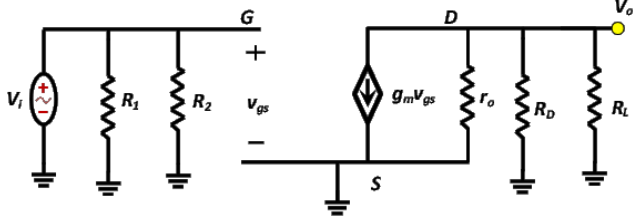
\includegraphics[width=\linewidth]{exp1cktac}
		\caption{}
		\label{fig:exp1cktac}
	\end{subfigure}
	\hfill
	\begin{subfigure}{0.14\textwidth}
		\centering
		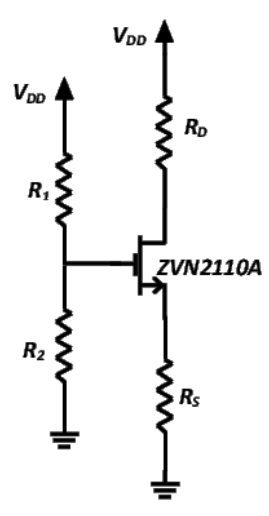
\includegraphics[width=\linewidth]{exp1cktdc}
		\caption{}
		\label{fig:exp1cktdc}
	\end{subfigure}
	\caption{Equivalent circuits for (a) small AC signals and (b) DC signals.}
\end{figure}
\vspace{-1em}
\begin{figure}[H]
	\centering
	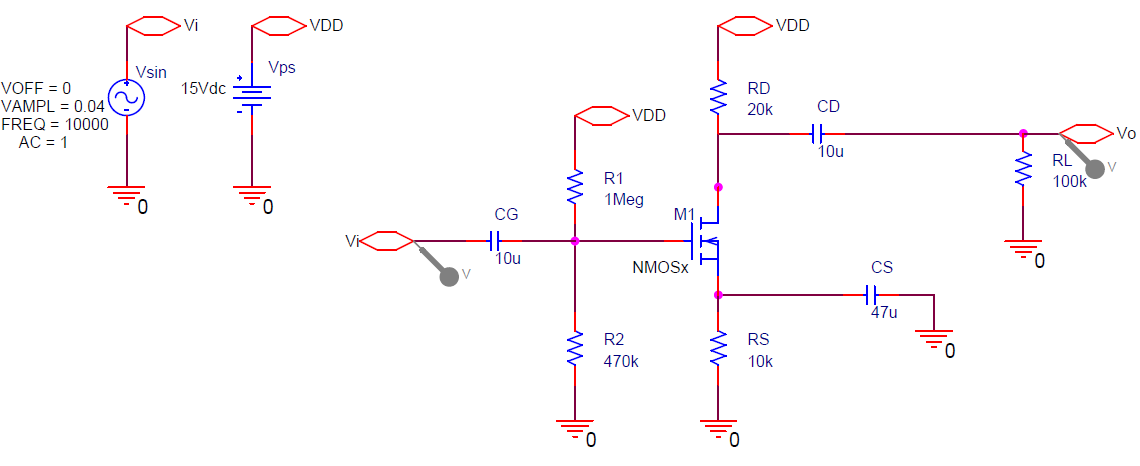
\includegraphics[width=0.8\linewidth]{exp1pspiceckt}
	\caption{Circuit in OrCAD for use in the AC sweep simulation.}
	\label{fig:exp1pspiceckt}
\end{figure}
\vspace{-1em}
\begin{figure}[H]
	\centering
	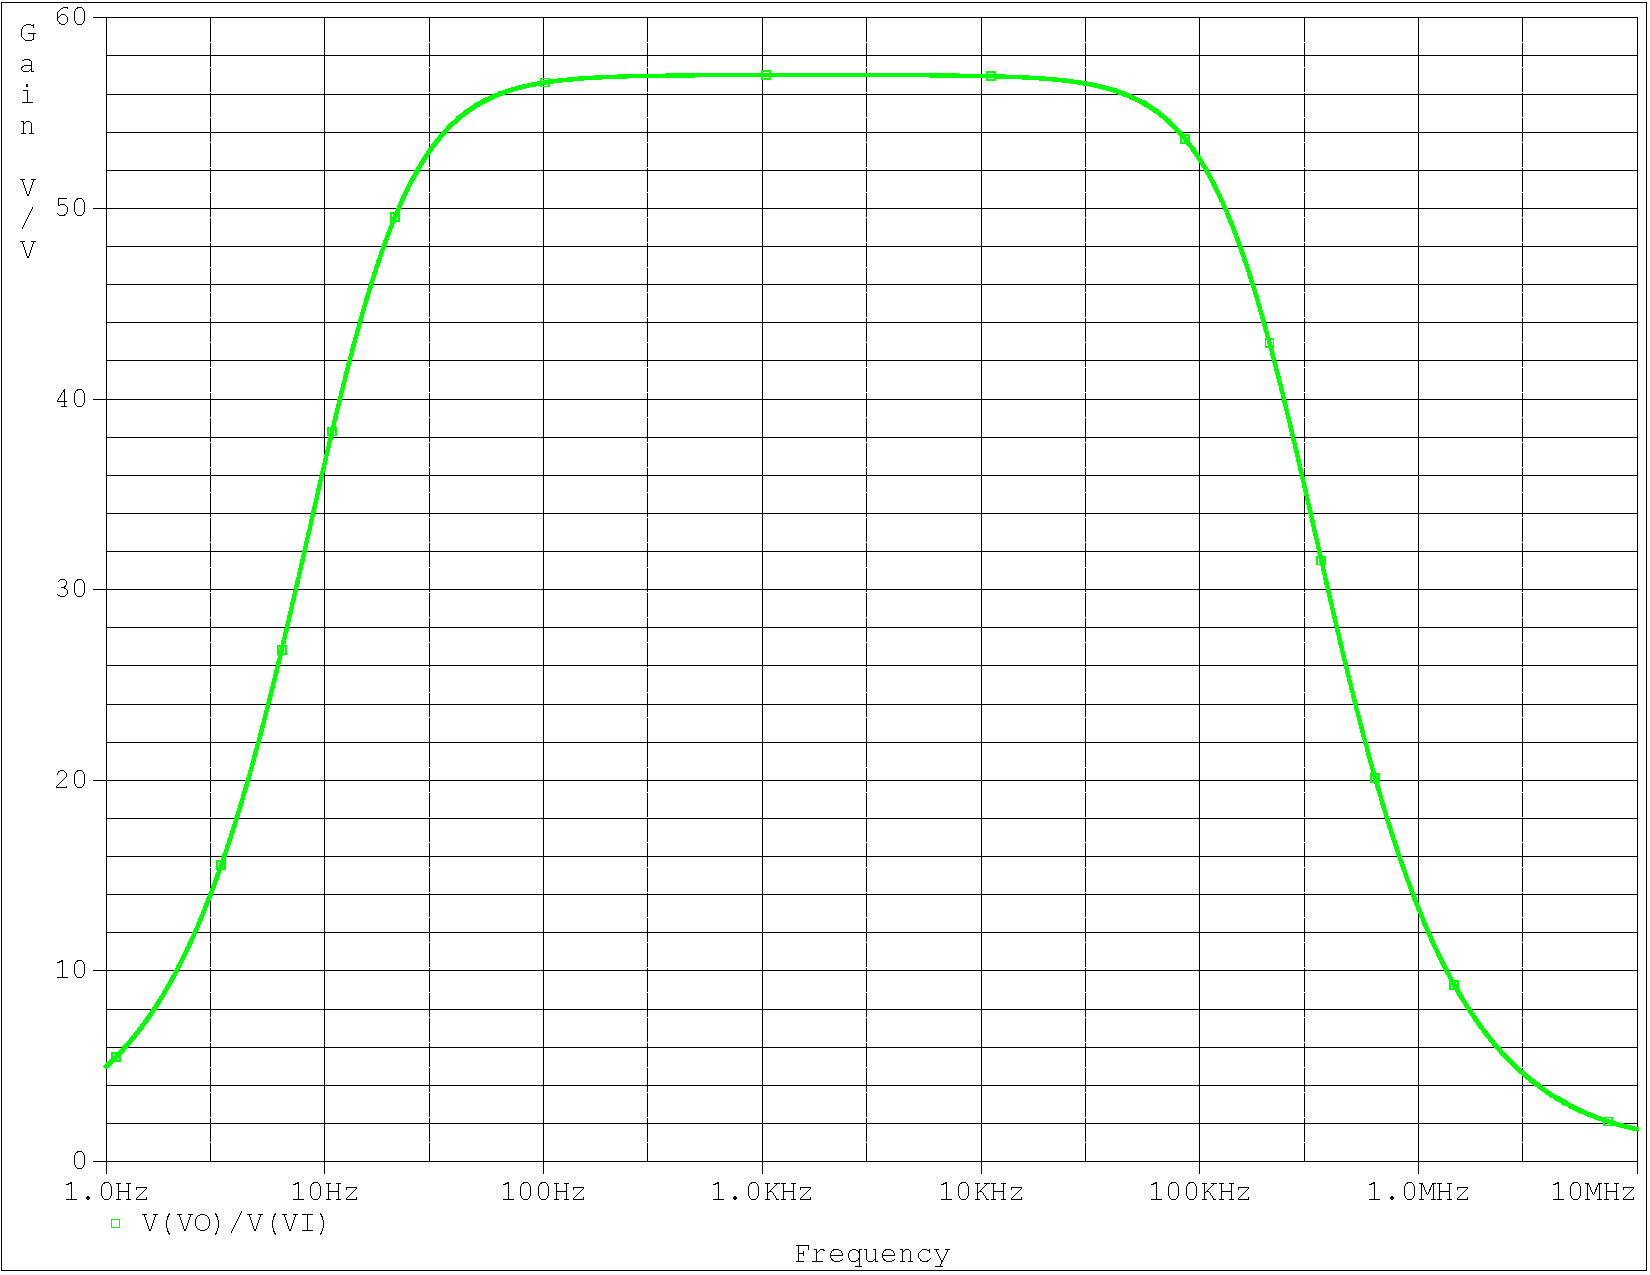
\includegraphics[width=0.7\linewidth]{exp1spice}
	\caption{Result of the PSPICE simulation using the modeled components.}
	\label{fig:exp1spice}
\end{figure}

\subsection{Procedure}
The follow steps were carried out, as instructed by the lab assignment.
\begin{enumerate}
	\item Using the chosen component values, the resistors were chosen and their resistances were measured using the DMM. The RLC meter was used to measure the capacitor values.
	\item The circuit was constructed and the DC power supply was attached. The capacitors were temporarily disconnected during this step. The terminal voltages were measured using the DMM. The transconductance was estimated using these values. 
	\item A \SI{20}{\mV} peak-to-peak sine input signal was applied using the function generator at \SI{20}{\kHz}. The output voltage was measured using the oscilloscope. The midband gain was calculated. The resistance was adjusted to adjust the current, affecting the gain of the amplifier.
	\item The low and high cutoff frequencies were found by calculating $0.707 \times$ the midband gain. 
	\item The frequency response of the amplifier was plotted using Excel. 
	\item The amplitude of the input signal was increased until clipping was observed and snapshots were taken of the oscilloscope. The drain voltage was measured using the oscilloscope with DC coupling.
\end{enumerate}

\subsection{Results and analysis}
% state all measured values, graphs, tables, and figs.
% state any deviation from theoretical expected values
% use tables and graphs
% * must justify error in results otherwise the experiment failed

\subsubsection{Component and DC measurements}
The resistors were measured using the DMM and the capacitors were measured with the RLC meter. These values were recorded in Table \ref{table:lab1components}.
\begin{table}[H]
	\centering
	\caption{Experimental and nominal component values.}
	\label{table:lab1components}
	\begin{threeparttable}
		\begin{tabular}{cccc}
			\toprule
			Component & Nominal & Experimental & \% Error  \\
			\midrule
			$R_1$ & \SI{1}{\Mohm} & \SI{1.01}{\Mohm} & 1\% \\
			$R_2$ & \SI{470}{\kohm} & \SI{465}{\kohm} & 1\% \\
			$R_D$ & \SI{20}{\kohm} & \SI{19.47}{\kohm} & 2.6\% \\
			$R_S$ & \SI{10}{\kohm} & \SI{9.75}{\kohm} & 2.5\% \\
			$C_D$ & \SI{10}{\micro\farad} & \SI{9.77}{\micro\farad} & 2.3\% \\
			$C_G$ & \SI{10}{\micro\farad} & \SI{9.56}{\micro\farad} & 4.4\% \\
			$C_S$ & \SI{47}{\micro\farad} & \SI{38.4}{\micro\farad} & 18.3\% \\
			$R_L$ & \SI{100}{\kohm} & \SI{97.3}{\kohm} & 2.7\% \\
			\bottomrule
		\end{tabular}
	\end{threeparttable}
\end{table}
With no AC input signal, the transistor terminal voltages were measured using the DMM. The source, gate, and drain voltages were respectively, \begin{align*}
	V_S & = \SI{3.195}{\V} \\
	V_G & = \SI{4.568}{\V} \\
	V_D & = \SI{8.622}{\V}
\end{align*}
With these component values, the input signal was applied and the output voltage was measured as \SI{1.4}{\V} with an input voltage of \SI{20}{\mV} peak-to-peak sine wave. The gain was calculated to be \SI{70}{\V/\V}, roughly 20\% higher than the maximum allowed voltage. Adjusting $R_S$ to \SI{20}{\kohm} dropped the gain below the minimum, at \SI{35}{\V/\V}. Choosing a resistance between these, $R_S$ was trimmed up to \SI{16.8}{\kohm}. With an input peak-to-peak voltage of \SI{20.4}{\mV}, the output voltage was measured at \SI{912}{\mV}---a gain of \SI{-44.7}{\V/\V}. With the new resistance, the DC voltages were remeasured, \begin{align*}
	V_S & = \SI{3.220}{\V} \\
	V_G & = \SI{4.566}{\V} \\
	V_D & = \SI{10.69}{\V}
\end{align*}
This change brought the drain current and transconductance to \begin{align*}
	I_D & = \frac{\SI{3.220}{\V}}{\SI{16.4}{\kohm}} = \SI{0.196}{\mA} \\
	g_m & = \sqrt{2 k_n I_D} = \SI{2.8}{\mA/\V}
\end{align*}
The cutoff frequencies were found by sweeping the frequency until the output voltage reached $0.707 \times \SI{912}{\mV}$. Using the oscilloscope, the output voltages were measured and shown in Figure \ref{fig:exp1f}. The low and high cutoff frequencies were determined to be $f_L = \SI{41}{\Hz}$ and $f_H= \SI{260}{\kHz}$. Additional points were collected at various frequencies, sweeping from \SI{20}{\Hz} to \SI{500}{\kHz}. This data was collected using Excel and plotted in Figure \ref{fig:exp1freq}.

Next, the clipping was investigated by varying the amplitude of the input signal at \SI{10}{\kHz}. It was found that the bottom of the output signal was clipped first, albeit the entire waveform was distorted. Using cursors, the clipping was measured at $V_\mathrm{min} = \SI{3.6}{\V}$ and $V_\mathrm{max} = \SI{14.2}{\V}$.

\subsection{Conclusion}
%  conclusion of the exp
We achieved the required gain for the single stage common source amplifier. The overall error in the midband gain was roughly 10.6\% lower than expectation, but within the 20\% tolerance. The amplifier designed in the experiment had a usable bandwidth of roughly \SI{260}{\kHz}. The input resistance exceeded the requirement of only \SI{200}{\kohm}. The measured values roughly fit the expected response, found using the PSPICE simulation.

\begin{figure}[H]
	\centering
	\begin{subfigure}{0.4\linewidth}
		\centering
		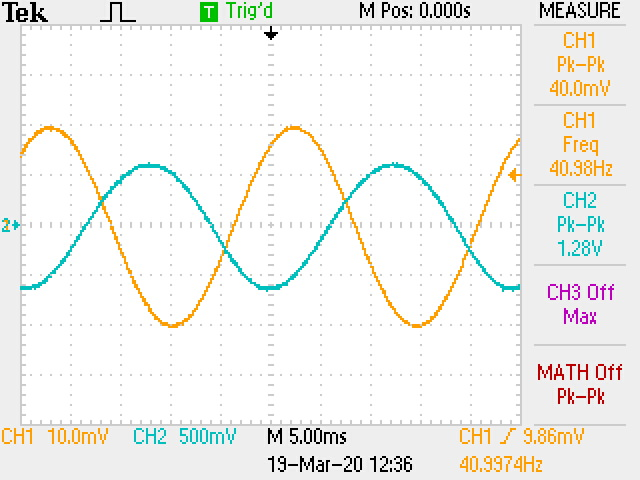
\includegraphics[width=\linewidth]{exp1fl}
		\caption{Low frequency cutoff.}
		\label{fig:exp1fl}
	\end{subfigure}
	\hfill
	\begin{subfigure}{0.4\linewidth}
		\centering
		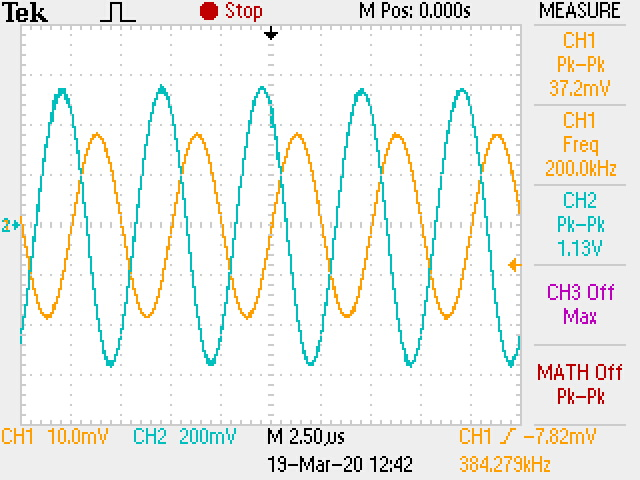
\includegraphics[width=\linewidth]{exp1fh}
		\caption{High frequency cutoff.}
		\label{fig:exp1fh}
	\end{subfigure}
	\caption{Cutoff frequencies measured using the oscilloscope.}
	\label{fig:exp1f}
\end{figure}
\vspace{-2em}
\begin{figure}[H]
	\centering
	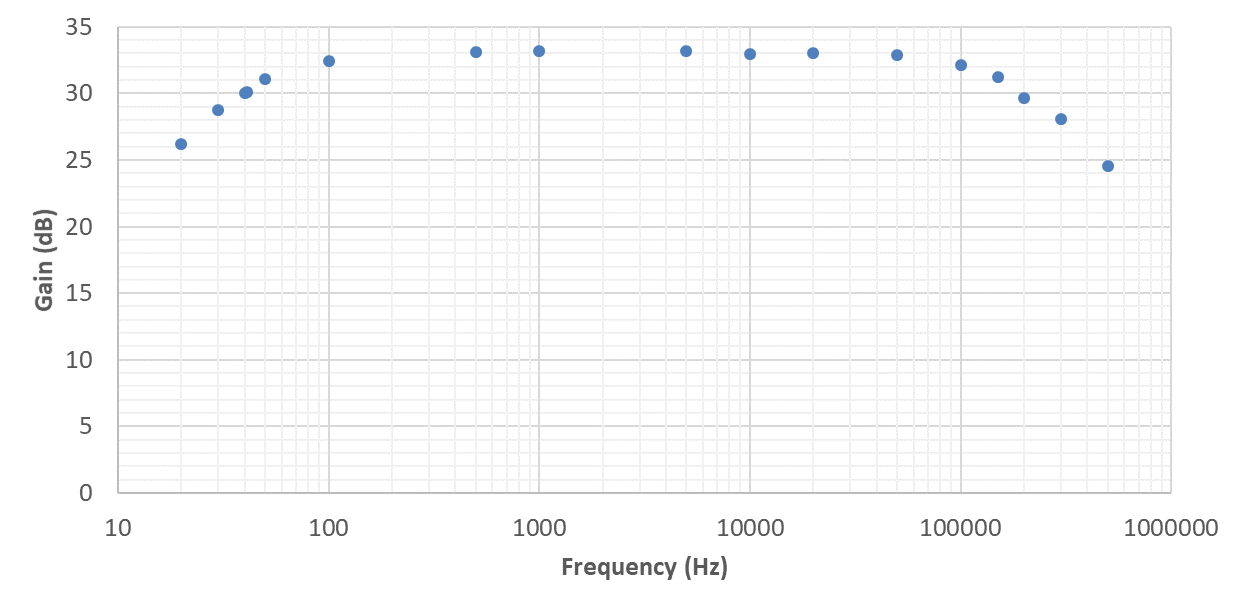
\includegraphics[width=0.9\linewidth]{exp1freq}
	\caption{The frequency response of the amplifier.}
	\label{fig:exp1freq}
\end{figure}

\pagebreak

%%%%%%%%%%%%%%%%%%%%%%%%%%%%%%%%%%%%%%%%%%%%%%%%%%%%%%%%%%%%%
\section{Current mirror circuit}

\subsection{Purpose}
% purpose of the experiment and its specs and/or design requirements
The purpose of this experiment is to design and implement a current circuit mirror using a matched NMOS transistors on the CD4007 IC. This circuit produces an equal current across a matched transistor with a connected gate. This experiment demonstrates a use-case for matched transistors.

\subsection{Theoretical background}
% background and its theory of operation, circuit diagrams, the main equations, results from the prelab
A current mirror circuit creates a current source that mirrors the current through a matched transistor. In this experiment, we will use matched NMOS transistors using the CD4007 chip. The current mirror circuit used in this experiment is shown in Figure \ref{fig:exp2ckt} below.

\begin{figure}[H]
	\centering
	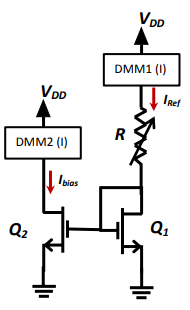
\includegraphics[width=0.2\linewidth]{exp2ckt}
	\caption{The current mirror circuit used in Experiment 2.}
	\label{fig:exp2ckt}
\end{figure}
In order to achieve a reference current of \SI{1}{\mA} through $Q_1$, the resistor value needs to be calculated. As the transistor will be operating within the saturation region, we can determine the gate-source voltage required.
\begin{align*}
	I_D & \approx \frac{k_n}{2} \left(V_{GS} - V_t\right)^2  \\
	\SI{1}{\mA} & \approx \frac{0.08}{2} \left( V_{GS} - \SI{1.7}{\V}\right)^2 \\
	V_{GS} & \approx \SI{1.86}{\V}
\end{align*}
As the source is connected to ground, the gate-source voltage is equivalent to the gate and drain voltages. From this, the resistance can be calculated as \begin{align*}
	R & = \frac{V_{DD} - V_G}{I} = \frac{5 - 1.86 \; \si{\V}}{1 \; \si{\mA}} \\
		& = \SI{3.14}{\kohm}
\end{align*}

\pagebreak
\subsection{Procedure}
The follow steps were carried out, as instructed by the lab assignment.
\begin{enumerate}
	\item The circuit shown in Figure \ref{fig:exp2ckt} was constructed using the CD4007 IC and a decade box as the variable resistor. The DC power supply was set to \SI{5}{\V} and the DMMs were attached to measure currents across each transistor.
	\item Pin 7 of the CD4007 was attached to ground, as it is attached to the bodies of each of the NFETs housed within the IC.
	%3383
	\item The decade box was initially set to the resistance found in the prelab (\SI{3.14}{\kohm}) and was varied until the reference current reached \SI{1}{\mA}.
	\item Both currents were measured with the DMM and recorded.
\end{enumerate}
%1 mA 2.110 mA
%1.477 3.123 mA

\subsection{Results and analysis}
% state all measured values, graphs, tables, and figs.
% state any deviation from theoretical expected values
% use tables and graphs
% * must justify error in results otherwise the experiment failed
The decade box achieved a reference current of \SI{1}{\mA} around \SI{3.38}{\kohm}, about 8\% higher than the expected value. This error is likely due to an inaccurate $k_n$ or $V_T$ value used in the prelab calculations. However, it was still in the rough order of magnitude.

At a reference current of \SI{1}{\mA}, the mirrored bias current was found to be \SI{2.110}{\mA}, around 5.5\% error from the expected \SI{2}{\mA}. This amount of error is fairly low and is due to defects in the manufacturing tolerances of the transistor aspect ratio of each transistor. The transistors are not perfectly matched and have some variances to them.
\subsection{Conclusion}
%  conclusion of the exp
The current mirror circuit is used to create a current source through a transistor, equal to that of a matching and connected transistor. In this experiment, we were able to create this with roughly 5\% error, within the expected tolerance of the matched NMOS transistors in the CD4007 IC.

\pagebreak
%%%%%%%%%%%%%%%%%%%%%%%%%%%%%%%%%%%%%%%%%%%%%%%%%%%%%%%%%%%%%
\section{CMOS Inverter}

\subsection{Purpose}
% purpose of the experiment and its specs and/or design requirements
This experiment uses a CMOS chip, containing an NMOS and PMOS, to create a logic inverter. We use these transistors to invert a signal from `off' to `on' and vice-versa. In between these boolean regions, one or both may operate in the saturation region and can act as a CMOS inverting amplifier with a relatively high gain. 

\subsection{Theoretical background}
% background and its theory of operation, circuit diagrams, the main equations, results from the prelab
On a CMOS chip, it will contain two complementary transistors: one PMOS and one NMOS transistor. Here, we will each transistor with the gates connected to a common node. If we use discrete logic levels, containing a logic low (\SI{0}{\V}) and logic high (\SI{5}{\V}), each transistor acts as a switch in the triode region. However, at transitioning voltages, each transistor goes through the saturation region and acts as an amplifier circuit.

In this experiment, we will build the inverter circuit shown in Figure \ref{fig:exp3ckt} below. As we increase the input voltage $V_i$, it will cycle through the five regions shown in Figure \ref{fig:exp3regions}. At an output voltage half of the supply voltage, in region 3, the inverter can act as an inverting amplifier. We will explore this using the function generator in this experiment.

\begin{figure}[h]
	\centering
	\begin{subfigure}{0.25\linewidth}
		\centering
		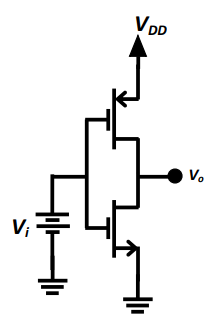
\includegraphics[width=\linewidth]{exp3ckt}
		\caption{}
		\label{fig:exp3ckt}
	\end{subfigure}
	\hfill
	\begin{subfigure}{0.65\linewidth}
		\centering
		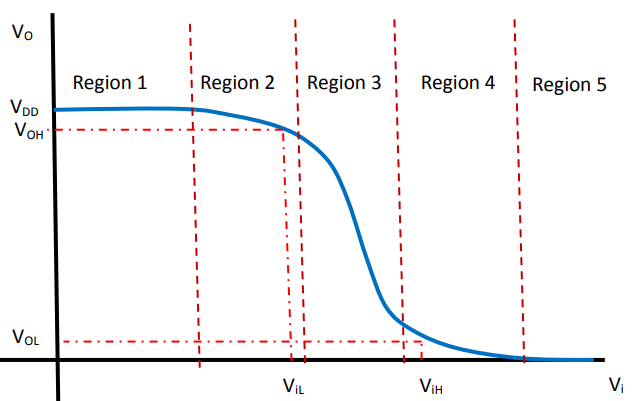
\includegraphics[width=\linewidth]{exp3regions}
		\caption{}
		\label{fig:exp3regions}
	\end{subfigure}
	\caption{The CMOS inverter (a) circuit and (b) the corresponding operating regions.}
\end{figure}

\subsection{Procedure}
The follow steps were carried out, as instructed by the lab assignment.
\begin{enumerate}
	\item The circuit shown in Figure \ref{fig:exp3ckt} was constructed using the CMOS pair Q2 within the CD4007 IC. One DC power supply $V_{DD}$ was set to \SI{5}{\V}. The other will be used as the input gate voltage.
	\item The NFET base pins were grounded using Pin 7, and the PFET bases were tied to $V_{DD}$.
	\item The input voltage $V_i$ was swept from \num{0} to \SI{5}{\V}. DMMs were used to measure the input and output voltages. These points were recorded in Excel and the output-input voltage characteristics were plotted.
	\item The five transition regions were determined on the plot.
	\item The input voltage at an output voltage of $V_{DD}/2=2.5$ was recorded. The function generator was enabled with an offset voltage of this value using \SI{10}{\mV} peak-to-peak sine waves at \SI{1}{\kHz}.
	\item Using the oscilloscope with AC coupling, the output voltage was measured and the gain was calculated. A screenshot was taken at this point.
\end{enumerate}

\subsection{Results and analysis}
% state all measured values, graphs, tables, and figs.
% state any deviation from theoretical expected values
% use tables and graphs
% * must justify error in results otherwise the experiment failed

After sweeping the input voltage from \SI{0}{\V} to \SI{5}{\V}, the data was recorded and plotted. We can estimate the regions by using a threshold voltage of $V_{tn} \approx \SI{1.6}{\V}$ and $V_{tp} \approx \SI{-2.25}{\V}$ and applying the cutoff/triode/saturation conditions to each transistor to determine the region transitions. The results of this are shown in Figure \ref{fig:exp3coloredregions} below.


% 2.057, out = 2.512 V
In region 3, at an input voltage $V_i \approx \SI{2.0574}{\V}$, the output voltage is roughly $V_{DD}/2=\SI{2.50}{\V}$. At this point, the CMOS pair acts as an amplifier as both transistors are in the saturation region. We can apply a \SI{10}{\mV} sine wave using the function generator at this voltage offset to calculate the gain. For an input of \SI{6.96}{\mV}, the output was \SI{320}{\mV}, shown in Figure \ref{fig:exp3scope} below. This was a gain of \SI{45.98}{\V/\V}.

\subsection{Conclusion}
%  conclusion of the exp
In this experiment, we successfully used the CMOS inverter to invert a \SI{5}{\V} input. By sweeping the input voltage, we verified the five regions which the inverter can operate as one or both transistors run through the triode and saturation region. When both transistors are within the saturation region, we found the inverter can act as an inverting amplifier, with a gain of nearly \SI{50}{\V/\V}.

\begin{figure}[H]
	\centering
	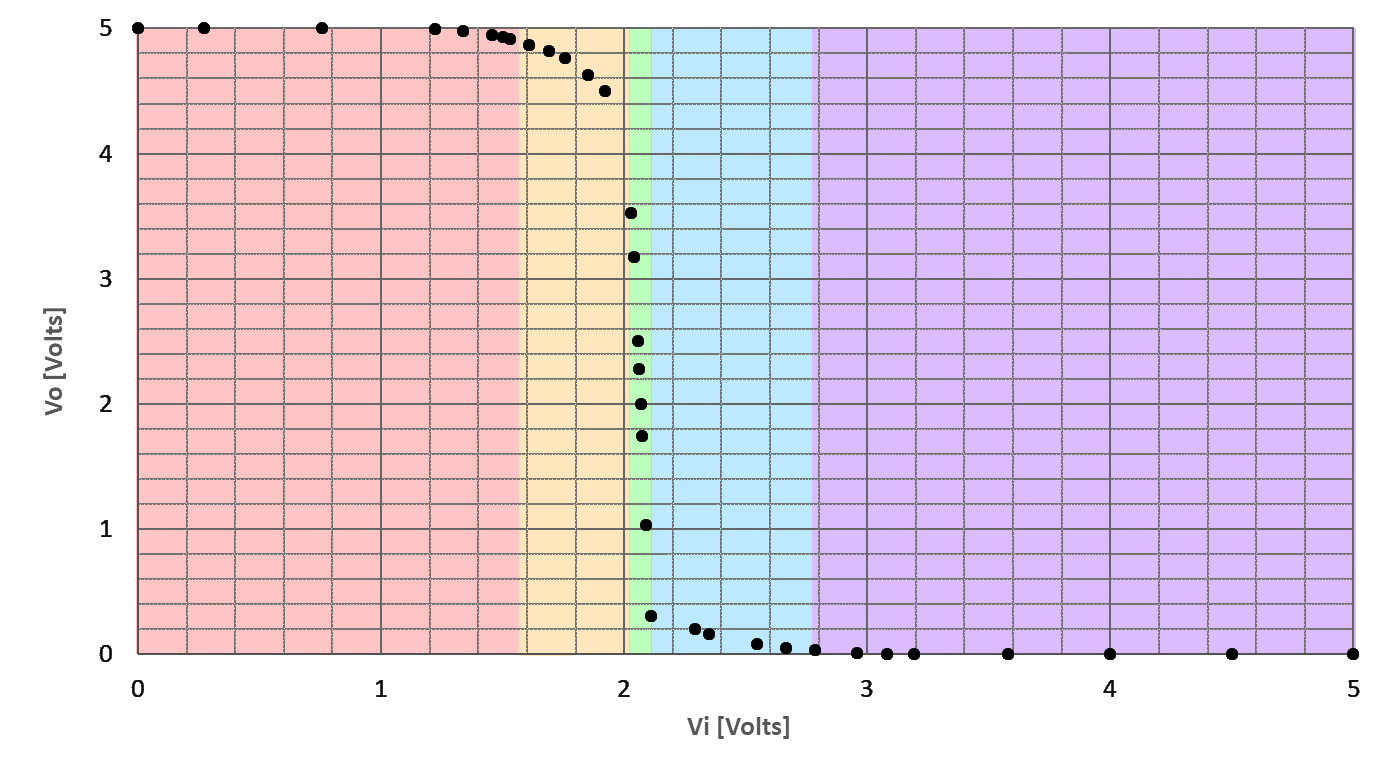
\includegraphics[width=0.9\linewidth]{exp3coloredregions}
	\caption{The regions of the CMOS inverter. (1) red, (2) orange, (3) green, (4) blue, (5) purple.}
	\label{fig:exp3coloredregions}
\end{figure}

\begin{figure}[H]
	\centering
	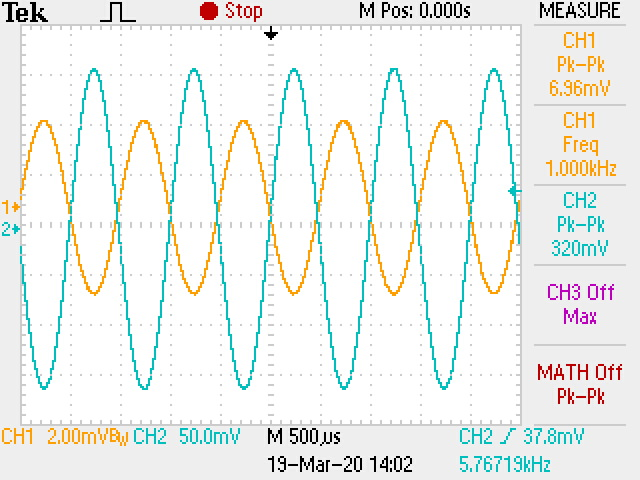
\includegraphics[width=0.4\linewidth]{exp3scope}
	\caption{CMOS inverter acting as an amplifier with a gain of nearly \SI{50}{\V/\V}.}
	\label{fig:exp3scope}
\end{figure}
\end{document}